% Options for packages loaded elsewhere
\PassOptionsToPackage{unicode}{hyperref}
\PassOptionsToPackage{hyphens}{url}
%
\documentclass[
]{article}
\usepackage{lmodern}
\usepackage{amssymb,amsmath}
\usepackage{ifxetex,ifluatex}
\ifnum 0\ifxetex 1\fi\ifluatex 1\fi=0 % if pdftex
  \usepackage[T1]{fontenc}
  \usepackage[utf8]{inputenc}
  \usepackage{textcomp} % provide euro and other symbols
\else % if luatex or xetex
  \usepackage{unicode-math}
  \defaultfontfeatures{Scale=MatchLowercase}
  \defaultfontfeatures[\rmfamily]{Ligatures=TeX,Scale=1}
\fi
% Use upquote if available, for straight quotes in verbatim environments
\IfFileExists{upquote.sty}{\usepackage{upquote}}{}
\IfFileExists{microtype.sty}{% use microtype if available
  \usepackage[]{microtype}
  \UseMicrotypeSet[protrusion]{basicmath} % disable protrusion for tt fonts
}{}
\makeatletter
\@ifundefined{KOMAClassName}{% if non-KOMA class
  \IfFileExists{parskip.sty}{%
    \usepackage{parskip}
  }{% else
    \setlength{\parindent}{0pt}
    \setlength{\parskip}{6pt plus 2pt minus 1pt}}
}{% if KOMA class
  \KOMAoptions{parskip=half}}
\makeatother
\usepackage{xcolor}
\IfFileExists{xurl.sty}{\usepackage{xurl}}{} % add URL line breaks if available
\IfFileExists{bookmark.sty}{\usepackage{bookmark}}{\usepackage{hyperref}}
\hypersetup{
  pdftitle={Single studies using the SelfControlledCaseSeries package},
  pdfauthor={Martijn J. Schuemie, Marc A. Suchard and Patrick Ryan},
  hidelinks,
  pdfcreator={LaTeX via pandoc}}
\urlstyle{same} % disable monospaced font for URLs
\usepackage[margin=1in]{geometry}
\usepackage{color}
\usepackage{fancyvrb}
\newcommand{\VerbBar}{|}
\newcommand{\VERB}{\Verb[commandchars=\\\{\}]}
\DefineVerbatimEnvironment{Highlighting}{Verbatim}{commandchars=\\\{\}}
% Add ',fontsize=\small' for more characters per line
\usepackage{framed}
\definecolor{shadecolor}{RGB}{248,248,248}
\newenvironment{Shaded}{\begin{snugshade}}{\end{snugshade}}
\newcommand{\AlertTok}[1]{\textcolor[rgb]{0.94,0.16,0.16}{#1}}
\newcommand{\AnnotationTok}[1]{\textcolor[rgb]{0.56,0.35,0.01}{\textbf{\textit{#1}}}}
\newcommand{\AttributeTok}[1]{\textcolor[rgb]{0.77,0.63,0.00}{#1}}
\newcommand{\BaseNTok}[1]{\textcolor[rgb]{0.00,0.00,0.81}{#1}}
\newcommand{\BuiltInTok}[1]{#1}
\newcommand{\CharTok}[1]{\textcolor[rgb]{0.31,0.60,0.02}{#1}}
\newcommand{\CommentTok}[1]{\textcolor[rgb]{0.56,0.35,0.01}{\textit{#1}}}
\newcommand{\CommentVarTok}[1]{\textcolor[rgb]{0.56,0.35,0.01}{\textbf{\textit{#1}}}}
\newcommand{\ConstantTok}[1]{\textcolor[rgb]{0.00,0.00,0.00}{#1}}
\newcommand{\ControlFlowTok}[1]{\textcolor[rgb]{0.13,0.29,0.53}{\textbf{#1}}}
\newcommand{\DataTypeTok}[1]{\textcolor[rgb]{0.13,0.29,0.53}{#1}}
\newcommand{\DecValTok}[1]{\textcolor[rgb]{0.00,0.00,0.81}{#1}}
\newcommand{\DocumentationTok}[1]{\textcolor[rgb]{0.56,0.35,0.01}{\textbf{\textit{#1}}}}
\newcommand{\ErrorTok}[1]{\textcolor[rgb]{0.64,0.00,0.00}{\textbf{#1}}}
\newcommand{\ExtensionTok}[1]{#1}
\newcommand{\FloatTok}[1]{\textcolor[rgb]{0.00,0.00,0.81}{#1}}
\newcommand{\FunctionTok}[1]{\textcolor[rgb]{0.00,0.00,0.00}{#1}}
\newcommand{\ImportTok}[1]{#1}
\newcommand{\InformationTok}[1]{\textcolor[rgb]{0.56,0.35,0.01}{\textbf{\textit{#1}}}}
\newcommand{\KeywordTok}[1]{\textcolor[rgb]{0.13,0.29,0.53}{\textbf{#1}}}
\newcommand{\NormalTok}[1]{#1}
\newcommand{\OperatorTok}[1]{\textcolor[rgb]{0.81,0.36,0.00}{\textbf{#1}}}
\newcommand{\OtherTok}[1]{\textcolor[rgb]{0.56,0.35,0.01}{#1}}
\newcommand{\PreprocessorTok}[1]{\textcolor[rgb]{0.56,0.35,0.01}{\textit{#1}}}
\newcommand{\RegionMarkerTok}[1]{#1}
\newcommand{\SpecialCharTok}[1]{\textcolor[rgb]{0.00,0.00,0.00}{#1}}
\newcommand{\SpecialStringTok}[1]{\textcolor[rgb]{0.31,0.60,0.02}{#1}}
\newcommand{\StringTok}[1]{\textcolor[rgb]{0.31,0.60,0.02}{#1}}
\newcommand{\VariableTok}[1]{\textcolor[rgb]{0.00,0.00,0.00}{#1}}
\newcommand{\VerbatimStringTok}[1]{\textcolor[rgb]{0.31,0.60,0.02}{#1}}
\newcommand{\WarningTok}[1]{\textcolor[rgb]{0.56,0.35,0.01}{\textbf{\textit{#1}}}}
\usepackage{graphicx,grffile}
\makeatletter
\def\maxwidth{\ifdim\Gin@nat@width>\linewidth\linewidth\else\Gin@nat@width\fi}
\def\maxheight{\ifdim\Gin@nat@height>\textheight\textheight\else\Gin@nat@height\fi}
\makeatother
% Scale images if necessary, so that they will not overflow the page
% margins by default, and it is still possible to overwrite the defaults
% using explicit options in \includegraphics[width, height, ...]{}
\setkeys{Gin}{width=\maxwidth,height=\maxheight,keepaspectratio}
% Set default figure placement to htbp
\makeatletter
\def\fps@figure{htbp}
\makeatother
\setlength{\emergencystretch}{3em} % prevent overfull lines
\providecommand{\tightlist}{%
  \setlength{\itemsep}{0pt}\setlength{\parskip}{0pt}}
\setcounter{secnumdepth}{5}

\title{Single studies using the SelfControlledCaseSeries package}
\author{Martijn J. Schuemie, Marc A. Suchard and Patrick Ryan}
\date{2020-06-19}

\begin{document}
\maketitle

{
\setcounter{tocdepth}{2}
\tableofcontents
}
\hypertarget{introduction}{%
\section{Introduction}\label{introduction}}

This vignette describes how you can use the
\texttt{SelfControlledCaseSeries} package to perform a single
Self-Controlled Case Series (SCCS) study. We will walk through all the
steps needed to perform an exemplar study, and we have selected the
well-studied topic of the effect of NSAIDs on gastrointestinal (GI)
bleeding-related hospitalization. For simplicity, we focus on one NSAID:
diclofenac.

\hypertarget{installation-instructions}{%
\section{Installation instructions}\label{installation-instructions}}

Before installing the \texttt{SelfControlledCaseSeries} package make
sure you have Java available. For Windows users, RTools is also
necessary. See \href{https://ohdsi.github.io/Hades/rSetup.html}{these
instructions} for properly configuring your R environment.

The \texttt{SelfControlledCaseSeries} package is maintained in a
\href{https://github.com/OHDSI/SelfControlledCaseSeries}{Github
repository}, and can be downloaded and installed from within R using the
\texttt{remotes} package:

\begin{Shaded}
\begin{Highlighting}[]
\KeywordTok{install.packages}\NormalTok{(}\StringTok{"remotes"}\NormalTok{)}
\KeywordTok{library}\NormalTok{(remotes)}
\KeywordTok{install_github}\NormalTok{(}\StringTok{"ohdsi/SelfControlledCaseSeries"}\NormalTok{) }
\end{Highlighting}
\end{Shaded}

Once installed, you can type \texttt{library(SelfControlledCaseSeries)}
to load the package.

\hypertarget{overview}{%
\section{Overview}\label{overview}}

In the \texttt{SelfControlledCaseSeries} package a study requires at
least three steps:

\begin{enumerate}
\def\labelenumi{\arabic{enumi}.}
\item
  Loading the necessary data from the database.
\item
  Transforming the data into a format suitable for an SCCS study. This
  step includes the creation of covariates based on the variables
  extracted from the database, such as defining risk windows based on
  exposures. It also includes transforming the data into non-overlapping
  time intervals, with information on the various covariates and
  outcomes per interval.
\item
  Fitting the model using conditional Poisson regression.
\end{enumerate}

In the following sections these steps will be demonstrated for
increasingly complex studies.

\hypertarget{studies-with-a-single-drug}{%
\section{Studies with a single drug}\label{studies-with-a-single-drug}}

\hypertarget{configuring-the-connection-to-the-server}{%
\subsection{Configuring the connection to the
server}\label{configuring-the-connection-to-the-server}}

We need to tell R how to connect to the server where the data are.
\texttt{SelfControlledCaseSeries} uses the \texttt{DatabaseConnector}
package, which provides the \texttt{createConnectionDetails} function.
Type \texttt{?createConnectionDetails} for the specific settings
required for the various database management systems (DBMS). For
example, one might connect to a PostgreSQL database using this code:

\begin{Shaded}
\begin{Highlighting}[]
\NormalTok{connectionDetails <-}\StringTok{ }\KeywordTok{createConnectionDetails}\NormalTok{(}\DataTypeTok{dbms =} \StringTok{"postgresql"}\NormalTok{, }
                                             \DataTypeTok{server =} \StringTok{"localhost/ohdsi"}\NormalTok{, }
                                             \DataTypeTok{user =} \StringTok{"joe"}\NormalTok{, }
                                             \DataTypeTok{password =} \StringTok{"supersecret"}\NormalTok{)}

\NormalTok{cdmDatabaseSchema <-}\StringTok{ "my_cdm_data"}
\NormalTok{cohortDatabaseSchema <-}\StringTok{ "my_results"}
\NormalTok{cdmVersion <-}\StringTok{ "5"}
\end{Highlighting}
\end{Shaded}

The last three lines define the \texttt{cdmDatabaseSchema} and
\texttt{cohortDatabaseSchema} variables,as well as the CDM version.
We'll use these later to tell R where the data in CDM format live, where
we have stored our cohorts of interest, and what version CDM is used.
Note that for Microsoft SQL Server, databaseschemas need to specify both
the database and the schema, so for example
\texttt{cdmDatabaseSchema\ \textless{}-\ "my\_cdm\_data.dbo"}.

\hypertarget{preparing-the-health-outcome-of-interest}{%
\subsection{Preparing the health outcome of
interest}\label{preparing-the-health-outcome-of-interest}}

We need to define the exposures and outcomes for our study. One way to
do this is by writing SQL statements against the OMOP CDM that populate
a table of events in which we are interested. The resulting table should
have the same structure as the \texttt{cohort} table in the CDM. This
means it should have the fields \texttt{cohort\_definition\_id},
\texttt{cohort\_start\_date}, \texttt{cohort\_end\_date}, and
\texttt{subject\_id}.

For our example study, we have created a file called \emph{vignette.sql}
with the following contents:

\begin{Shaded}
\begin{Highlighting}[]
\CommentTok{/***********************************}
\CommentTok{File vignette.sql }
\CommentTok{***********************************/}

\ControlFlowTok{IF}\NormalTok{ OBJECT_ID(}\StringTok{'@cohortDatabaseSchema.@outcomeTable'}\NormalTok{, }\StringTok{'U'}\NormalTok{) }\KeywordTok{IS} \KeywordTok{NOT} \KeywordTok{NULL}
  \KeywordTok{DROP} \KeywordTok{TABLE}\NormalTok{ @cohortDatabaseSchema.@outcomeTable;}

\KeywordTok{SELECT} \DecValTok{1} \KeywordTok{AS}\NormalTok{ cohort_definition_id,}
\NormalTok{    condition_start_date }\KeywordTok{AS}\NormalTok{ cohort_start_date,}
\NormalTok{    condition_end_date }\KeywordTok{AS}\NormalTok{ cohort_end_date,}
\NormalTok{    condition_occurrence.person_id }\KeywordTok{AS}\NormalTok{ subject_id}
\KeywordTok{INTO}\NormalTok{ @cohortDatabaseSchema.@outcomeTable}
\KeywordTok{FROM}\NormalTok{ @cdmDatabaseSchema.condition_occurrence}
\KeywordTok{INNER} \KeywordTok{JOIN}\NormalTok{ @cdmDatabaseSchema.visit_occurrence}
    \KeywordTok{ON}\NormalTok{ condition_occurrence.visit_occurrence_id }\OperatorTok{=}\NormalTok{ visit_occurrence.visit_occurrence_id}
\KeywordTok{WHERE}\NormalTok{ condition_concept_id }\KeywordTok{IN}\NormalTok{ (}
        \KeywordTok{SELECT}\NormalTok{ descendant_concept_id}
        \KeywordTok{FROM}\NormalTok{ @cdmDatabaseSchema.concept_ancestor}
        \KeywordTok{WHERE}\NormalTok{ ancestor_concept_id }\OperatorTok{=} \DecValTok{192671} \CommentTok{-- GI - Gastrointestinal haemorrhage}
\NormalTok{        )}
    \KeywordTok{AND}\NormalTok{ visit_occurrence.visit_concept_id }\KeywordTok{IN}\NormalTok{ (}\DecValTok{9201}\NormalTok{, }\DecValTok{9203}\NormalTok{);}
\end{Highlighting}
\end{Shaded}

This is parameterized SQL which can be used by the \texttt{SqlRender}
package. We use parameterized SQL so we do not have to pre-specify the
names of the CDM and cohort schemas. That way, if we want to run the SQL
on a different schema, we only need to change the parameter values; we
do not have to change the SQL code. By also making use of translation
functionality in \texttt{SqlRender}, we can make sure the SQL code can
be run in many different environments.

\begin{Shaded}
\begin{Highlighting}[]
\KeywordTok{library}\NormalTok{(SqlRender)}
\NormalTok{sql <-}\StringTok{ }\KeywordTok{readSql}\NormalTok{(}\StringTok{"vignette.sql"}\NormalTok{)}
\NormalTok{sql <-}\StringTok{ }\KeywordTok{render}\NormalTok{(sql,}
              \DataTypeTok{cdmDatabaseSchema =}\NormalTok{ cdmDatabaseSchema, }
              \DataTypeTok{cohortDatabaseSchema =}\NormalTok{ cohortDatabaseSchema}
              \DataTypeTok{outcomeTable =} \StringTok{"my_outcomes"}\NormalTok{)}
\NormalTok{sql <-}\StringTok{ }\KeywordTok{translate}\NormalTok{(sql, }\DataTypeTok{targetDialect =}\NormalTok{ connectionDetails}\OperatorTok{$}\NormalTok{dbms)}

\NormalTok{connection <-}\StringTok{ }\KeywordTok{connect}\NormalTok{(connectionDetails)}
\KeywordTok{executeSql}\NormalTok{(connection, sql)}
\end{Highlighting}
\end{Shaded}

In this code, we first read the SQL from the file into memory. In the
next line, we replace the three parameter names with the actual values.
We then translate the SQL into the dialect appropriate for the DBMS we
already specified in the \texttt{connectionDetails}. Next, we connect to
the server, and submit the rendered and translated SQL.

If all went well, we now have a table with the outcome of interest. We
can see how many events:

\begin{Shaded}
\begin{Highlighting}[]
\NormalTok{sql <-}\StringTok{ }\KeywordTok{paste}\NormalTok{(}\StringTok{"SELECT cohort_definition_id, COUNT(*) AS count"}\NormalTok{,}
             \StringTok{"FROM @cohortDatabaseSchema.@outcomeTable"}\NormalTok{,}
             \StringTok{"GROUP BY cohort_definition_id"}\NormalTok{)}
\NormalTok{sql <-}\StringTok{ }\KeywordTok{render}\NormalTok{(sql, }
              \DataTypeTok{cohortDatabaseSchema =}\NormalTok{ cohortDatabaseSchema, }
              \DataTypeTok{outcomeTable =} \StringTok{"my_outcomes"}\NormalTok{)}
\NormalTok{sql <-}\StringTok{ }\KeywordTok{translate}\NormalTok{(sql, }\DataTypeTok{targetDialect =}\NormalTok{ connectionDetails}\OperatorTok{$}\NormalTok{dbms)}

\KeywordTok{querySql}\NormalTok{(connection, sql)}
\end{Highlighting}
\end{Shaded}

\begin{verbatim}
##   cohort_concept_id   count
## 1                 1 1029443
\end{verbatim}

\hypertarget{extracting-the-data-from-the-server}{%
\subsection{Extracting the data from the
server}\label{extracting-the-data-from-the-server}}

Now we can tell \texttt{SelfControlledCaseSeries} to extract all
necessary data for our analysis:

\begin{Shaded}
\begin{Highlighting}[]
\NormalTok{diclofenac <-}\StringTok{ }\DecValTok{1124300}

\NormalTok{sccsData <-}\StringTok{ }\KeywordTok{getDbSccsData}\NormalTok{(}\DataTypeTok{connectionDetails =}\NormalTok{ connectionDetails,}
                          \DataTypeTok{cdmDatabaseSchema =}\NormalTok{ cdmDatabaseSchema,}
                          \DataTypeTok{oracleTempSchema =}\NormalTok{ oracleTempSchema,}
                          \DataTypeTok{outcomeDatabaseSchema =}\NormalTok{ cohortDatabaseSchema,}
                          \DataTypeTok{outcomeTable =}\NormalTok{ outcomeTable,}
                          \DataTypeTok{outcomeIds =} \DecValTok{1}\NormalTok{,}
                          \DataTypeTok{exposureDatabaseSchema =}\NormalTok{ cdmDatabaseSchema,}
                          \DataTypeTok{exposureTable =} \StringTok{"drug_era"}\NormalTok{,}
                          \DataTypeTok{exposureIds =}\NormalTok{ diclofenac,}
                          \DataTypeTok{cdmVersion =}\NormalTok{ cdmVersion)}
\NormalTok{sccsData}
\end{Highlighting}
\end{Shaded}

\begin{verbatim}
## # SccsData object
## 
## Exposure cohort ID(s): 1124300
## Outcome cohort ID(s): 1
## 
## Inherits from Andromeda:
## # Andromeda object
## # Physical location:  C:\Users\MSCHUEMI\AppData\Local\Temp\RtmpiUzJm8\file23f86034105c.sqlite
## 
## Tables:
## $cases (observationPeriodId, caseId, personId, observationDays, startYear, startMonth, startDay, ageInDays, censoredDays, noninformativeEndCensor)
## $eraRef (eraType, eraId, eraName)
## $eras (eraType, caseId, eraId, value, startDay, endDay)
\end{verbatim}

There are many parameters, but they are all documented in the
\texttt{SelfControlledCaseSeries} manual. In short, we are pointing the
function to the table created earlier and indicating which cohort ID in
that table identifies the outcome. Note that it is possible to fetch the
data for multiple outcomes at once. We further point the function to the
\texttt{drug\_era} table, and specify the concept ID of our exposure of
interest: diclofenac. Again, note that it is also possible to fetch data
for multiple drugs at once. In fact, when we do not specify any exposure
IDs the function will retrieve the data for all the drugs found in the
\texttt{drug\_era} table.

All data about the patients, outcomes and exposures are extracted from
the server and stored in the \texttt{sccsData} object. This object uses
the \texttt{Andromeda} package to store information in a way that
ensures R does not run out of memory, even when the data are large.

We can use the generic \texttt{summary()} function to view some more
information of the data we extracted:

\begin{Shaded}
\begin{Highlighting}[]
\KeywordTok{summary}\NormalTok{(sccsData)}
\end{Highlighting}
\end{Shaded}

\begin{verbatim}
## SccsData object summary
## 
## Exposure cohort ID(s): 1124300
## Outcome cohort ID(s): 1
## 
## Outcome counts:
##   Outcome Subjects Outcome Events Outcome Observation Periods
## 1           457608        1029228                      464775
## 
## Eras:
## Number of era types: 2
## Number of eras: 1102342
\end{verbatim}

\hypertarget{saving-the-data-to-file}{%
\subsubsection{Saving the data to file}\label{saving-the-data-to-file}}

Creating the \texttt{sccsData} file can take considerable computing
time, and it is probably a good idea to save it for future sessions.
Because \texttt{sccsData} uses \texttt{Andromeda}, we cannot use R's
regular save function. Instead, we'll have to use the
\texttt{saveSccsData()} function:

\begin{Shaded}
\begin{Highlighting}[]
\KeywordTok{saveSccsData}\NormalTok{(sccsData, }\StringTok{"diclofenacAndGiBleed.zip"}\NormalTok{)}
\end{Highlighting}
\end{Shaded}

We can use the \texttt{loadSccsData()} function to load the data in a
future session.

\hypertarget{creating-the-study-population}{%
\subsection{Creating the study
population}\label{creating-the-study-population}}

From the data fetched from the server we can now define the population
we wish to study. If we retrieved data for multiple outcomes, we should
now select only one, and possibly impose further restrictions:

\begin{Shaded}
\begin{Highlighting}[]
\NormalTok{studyPop <-}\StringTok{ }\KeywordTok{createStudyPopulation}\NormalTok{(}\DataTypeTok{sccsData =}\NormalTok{ sccsData,}
                                  \DataTypeTok{outcomeId =} \DecValTok{1}\NormalTok{,}
                                  \DataTypeTok{firstOutcomeOnly =} \OtherTok{FALSE}\NormalTok{,}
                                  \DataTypeTok{naivePeriod =} \DecValTok{180}\NormalTok{)}
\end{Highlighting}
\end{Shaded}

Here we specify we wish to study the outcome with ID 1. Since this was
the only outcome for which we fetched the data, we could also have
skipped this argument. We furthermore specify that the first 180 days of
observation of every person, the so-called `naive period', will be
excluded from the analysis. Note that data in the naive period will be
used to determine exposure status at the start of follow-up (after the
end of the naive period). We also specify we will use all occurrences of
the outcome, not just the first one per person.

We can find out how many people (if any) were removed by any
restrictions we imposed:

\begin{Shaded}
\begin{Highlighting}[]
\KeywordTok{getAttritionTable}\NormalTok{(studyPop)}
\end{Highlighting}
\end{Shaded}

\begin{verbatim}
## # A tibble: 2 x 5
##   outcomeId description           outcomeSubjects outcomeEvents outcomeObsPeriods
##       <dbl> <chr>                           <dbl>         <dbl>             <dbl>
## 1         1 Outcomes                       457608       1029228            464775
## 2         1 180 days naive period          357183        821368            360559
\end{verbatim}

\hypertarget{defining-a-simple-model}{%
\subsection{Defining a simple model}\label{defining-a-simple-model}}

Next, we can use the data to define a simple model to fit:

\begin{Shaded}
\begin{Highlighting}[]
\NormalTok{covarDiclofenac <-}\StringTok{ }\KeywordTok{createEraCovariateSettings}\NormalTok{(}\DataTypeTok{label =} \StringTok{"Exposure of interest"}\NormalTok{,}
                                              \DataTypeTok{includeEraIds =}\NormalTok{ diclofenac,}
                                              \DataTypeTok{start =} \DecValTok{0}\NormalTok{,}
                                              \DataTypeTok{end =} \DecValTok{0}\NormalTok{,}
                                              \DataTypeTok{endAnchor =} \StringTok{"era end"}\NormalTok{)}

\NormalTok{sccsIntervalData <-}\StringTok{ }\KeywordTok{createSccsIntervalData}\NormalTok{(studyPop,}
\NormalTok{                                           sccsData,}
                                           \DataTypeTok{eraCovariateSettings =}\NormalTok{ covarDiclofenac)}

\KeywordTok{summary}\NormalTok{(sccsIntervalData)}
\end{Highlighting}
\end{Shaded}

\begin{verbatim}
## SccsIntervalData object summary
## 
## Outcome cohort ID: 1
## 
## Number of cases (observation periods): 33452
## Number of eras (spans of time): 66904
## Number of outcomes: 79710
## Number of covariates: 1
## Number of non-zero covariate values: 33452
\end{verbatim}

In this example, we use the \texttt{createEraCovariateSettings} to
define a single covariate: exposure to diclofenac. We specify that the
risk window is from start of exposure to the end by setting start and
end to 0, and defining the anchor for the end to be the era end, which
for drug eras is the end of exposure.

We then use the covariate definition in the
\texttt{createSccsIntervalData} function to generate the
\texttt{sccsIntervalData}. This represents the data in non-overlapping
time intervals, with information on the various covariates and outcomes
per interval.

\hypertarget{power-calculations}{%
\subsection{Power calculations}\label{power-calculations}}

Before we start fitting an outcome model, we might be interested to know
whether we have sufficient power to detect a particular effect size. It
makes sense to perform these power calculations once the study
population has been fully defined, so taking into account loss to the
various inclusion and exclusion criteria. This means we will use the
sccsIntervalData object we've just created as the basis for our power
calculations. Since the sample size is fixed in retrospective studies
(the data has already been collected), and the true effect size is
unknown, the SelfControlledCaseSeries package provides a function to
compute the minimum detectable relative risk (MDRR) instead:

\begin{Shaded}
\begin{Highlighting}[]
\KeywordTok{computeMdrr}\NormalTok{(sccsIntervalData,}
            \DataTypeTok{exposureCovariateId =} \DecValTok{1000}\NormalTok{,}
            \DataTypeTok{alpha =} \FloatTok{0.05}\NormalTok{,}
            \DataTypeTok{power =} \FloatTok{0.8}\NormalTok{,}
            \DataTypeTok{twoSided =} \OtherTok{TRUE}\NormalTok{,}
            \DataTypeTok{method =} \StringTok{"binomial"}\NormalTok{)}
\end{Highlighting}
\end{Shaded}

\begin{verbatim}
## # A tibble: 1 x 6
##   timeExposed timeTotal propTimeExposed propPopExposued events  mdrr
##         <dbl>     <dbl>           <dbl>           <dbl>  <dbl> <dbl>
## 1     3877887  74561262           0.052               1  79710  1.05
\end{verbatim}

Note that we have to provide the covariate ID of the exposure of
interest, which we learned by calling \texttt{summary} on
sccsIntervalData earlier. This is because we may have many covariates in
our model, but will likely only be interested in the MDRR of one.

\hypertarget{model-fitting}{%
\subsection{Model fitting}\label{model-fitting}}

The \texttt{fitSccsModel} function is used to fit the model:

\begin{Shaded}
\begin{Highlighting}[]
\NormalTok{model <-}\StringTok{ }\KeywordTok{fitSccsModel}\NormalTok{(sccsIntervalData)}
\end{Highlighting}
\end{Shaded}

We can inspect the resulting model:

\begin{Shaded}
\begin{Highlighting}[]
\NormalTok{model}
\end{Highlighting}
\end{Shaded}

\begin{verbatim}
## SccsModel object
## 
## Outcome ID: 1
## 
## Outcome count:
##   outcomeSubjects outcomeEvents outcomeObsPeriods
## 1          357183        821368            360559
## 
## Estimates:
## # A tibble: 1 x 7
##   Name                                ID Estimate LB95CI UB95CI logRr seLogRr
##   <chr>                            <dbl>    <dbl>  <dbl>  <dbl> <dbl>   <dbl>
## 1 Exposure of interest: Diclofenac  1000     1.26   1.22   1.29 0.228  0.0154
\end{verbatim}

This tells us what the estimated relative risk (the incidence rate
ratio) is during exposure to diclofenac compared to non-exposed time.

\hypertarget{adding-a-pre-exposure-window}{%
\subsection{Adding a pre-exposure
window}\label{adding-a-pre-exposure-window}}

The fact that NSAIDs like diclofenac can cause GI bleeds is well known
to doctors, and this knowledge affects prescribing behavior. For
example, a patient who has just had a GI bleed is not likely to be
prescribed diclofenac. This may lead to underestimation of the rate
during unexposed time, because the unexposed time includes time just
prior to exposure where observing of the outcome is unlikely because of
this behavior. One solution to this problem that is often used is to
introduce a separate `risk window' just prior to exposure, to separate
it from the remaining unexposed time. We can add such a `pre-exposure
window' to our analysis:

\begin{Shaded}
\begin{Highlighting}[]
\NormalTok{covarPreDiclofenac <-}\StringTok{ }\KeywordTok{createEraCovariateSettings}\NormalTok{(}\DataTypeTok{label =} \StringTok{"Pre-exposure"}\NormalTok{,}
                                                 \DataTypeTok{includeEraIds =}\NormalTok{ diclofenac,}
                                                 \DataTypeTok{start =} \DecValTok{-60}\NormalTok{,}
                                                 \DataTypeTok{end =} \DecValTok{-1}\NormalTok{,}
                                                 \DataTypeTok{endAnchor =} \StringTok{"era start"}\NormalTok{)}

\NormalTok{sccsIntervalData <-}\StringTok{ }\KeywordTok{createSccsIntervalData}\NormalTok{(}\DataTypeTok{studyPopulation =}\NormalTok{ studyPop,}
\NormalTok{                                           sccsData,}
                                           \DataTypeTok{eraCovariateSettings =} \KeywordTok{list}\NormalTok{(covarDiclofenac, }
\NormalTok{                                                                       covarPreDiclofenac))}

\NormalTok{model <-}\StringTok{ }\KeywordTok{fitSccsModel}\NormalTok{(sccsIntervalData)}
\end{Highlighting}
\end{Shaded}

Here we created a new covariate definition in addition to the first one.
We define the risk window to start 60 days prior to exposure, and end on
the day just prior to exposure. We combine the two covariate settings in
a list for the \texttt{createSccsIntervalData} function. Again, we can
take a look at the results:

\begin{Shaded}
\begin{Highlighting}[]
\NormalTok{model}
\end{Highlighting}
\end{Shaded}

\begin{verbatim}
## SccsModel object
## 
## Outcome ID: 1
## 
## Outcome count:
##   outcomeSubjects outcomeEvents outcomeObsPeriods
## 1          357183        821368            360559
## 
## Estimates:
## # A tibble: 2 x 7
##   Name                                ID Estimate LB95CI UB95CI   logRr seLogRr
##   <chr>                            <dbl>    <dbl>  <dbl>  <dbl>   <dbl>   <dbl>
## 1 Exposure of interest: Diclofenac  1000    1.25   1.21   1.29   0.225   0.0155
## 2 Pre-exposure: Diclofenac          1001    0.961  0.932  0.991 -0.0393  0.0157
\end{verbatim}

Here we indeed see a lower relative risk in the time preceding the
exposure, indicating the outcome might be a contra-indication for the
drug of interest.

\hypertarget{splitting-risk-windows}{%
\subsection{Splitting risk windows}\label{splitting-risk-windows}}

Often we will want to split the risk windows into smaller parts and
compute estimates for each part. This can give us insight into the
temporal distribution of the risk. We can add this to the model:

\begin{Shaded}
\begin{Highlighting}[]
\NormalTok{covarDiclofenacSplit <-}\StringTok{ }\KeywordTok{createEraCovariateSettings}\NormalTok{(}\DataTypeTok{label =} \StringTok{"Exposure of interest"}\NormalTok{,}
                                                   \DataTypeTok{includeEraIds =}\NormalTok{ diclofenac,}
                                                   \DataTypeTok{start =} \DecValTok{0}\NormalTok{,}
                                                   \DataTypeTok{end =} \DecValTok{0}\NormalTok{,}
                                                   \DataTypeTok{endAnchor =} \StringTok{"era end"}\NormalTok{,}
                                                   \DataTypeTok{splitPoints =} \KeywordTok{c}\NormalTok{(}\DecValTok{7}\NormalTok{, }\DecValTok{14}\NormalTok{))}

\NormalTok{covarPreDiclofenacSplit <-}\StringTok{ }\KeywordTok{createEraCovariateSettings}\NormalTok{(}\DataTypeTok{label =} \StringTok{"Pre-exposure"}\NormalTok{,}
                                                      \DataTypeTok{includeEraIds =}\NormalTok{ diclofenac,}
                                                      \DataTypeTok{start =} \DecValTok{-60}\NormalTok{,}
                                                      \DataTypeTok{end =} \DecValTok{-1}\NormalTok{,}
                                                      \DataTypeTok{endAnchor =} \StringTok{"era start"}\NormalTok{,}
                                                      \DataTypeTok{splitPoints =} \KeywordTok{c}\NormalTok{(}\OperatorTok{-}\DecValTok{30}\NormalTok{))}

\NormalTok{sccsIntervalData <-}\StringTok{ }\KeywordTok{createSccsIntervalData}\NormalTok{(}\DataTypeTok{studyPopulation =}\NormalTok{ studyPop,}
\NormalTok{                                           sccsData,}
                                           \DataTypeTok{eraCovariateSettings =} \KeywordTok{list}\NormalTok{(covarDiclofenacSplit,}
\NormalTok{                                                                       covarPreDiclofenacSplit))}
\end{Highlighting}
\end{Shaded}

Here we've redefined out covariate definitions: We kept the same start
and end dates, but enforced split points for the main exposure windows
at 7 and 14 days. For the pre-exposure window we divided the window into
two, at day 30 before the exposure start. Note that the split point
dates indicate the end date of the preceding part, so the exposure is
now split into day 0 to (and including) day 7, day 8 to (and including)
day 14, and day 15 until the end of exposure. The results are:

\begin{Shaded}
\begin{Highlighting}[]
\NormalTok{model}
\end{Highlighting}
\end{Shaded}

\begin{verbatim}
## SccsModel object
## 
## Outcome ID: 1
## 
## Outcome count:
##   outcomeSubjects outcomeEvents outcomeObsPeriods
## 1          357183        821368            360559
## 
## Estimates:
## # A tibble: 5 x 7
##   Name                                          ID Estimate LB95CI UB95CI    logRr seLogRr
##   <chr>                                      <dbl>    <dbl>  <dbl>  <dbl>    <dbl>   <dbl>
## 1 Exposure of interest: Diclofenac, day 0-7   1000    1.27   1.19   1.36   0.242    0.0355
## 2 Exposure of interest: Diclofenac, day 8-14  1001    1.42   1.31   1.53   0.351    0.0392
## 3 Exposure of interest: Diclofenac, day 15-   1002    1.22   1.17   1.26   0.196    0.0179
## 4 Pre-exposure: Diclofenac, day -60--30       1003    0.996  0.956  1.04  -0.00353  0.0209
## 5 Pre-exposure: Diclofenac, day -29-          1004    0.930  0.890  0.971 -0.0727   0.0223
\end{verbatim}

We see that the risk for the three exposure windows is more or less the
same, suggesting a constant risk. We also see that the period 60 to 30
days prior to exposure does not seem to show a decreased risk,
suggesting the effect of the contra-indication does not extend more than
30 days before the exposure.

\hypertarget{including-age-and-seasonality}{%
\subsection{Including age and
seasonality}\label{including-age-and-seasonality}}

Often both the rate of exposure and the outcome change with age, and can
even depend on the season. This may lead to confounding and may bias our
estimates. To correct for this we can include age and/or season into the
model.

For computational reasons we assume the effect of both age and season
are constant within each calendar month. We assume that the rate from
one month to the next can be different, but we also assume that
subsequent months have somewhat similar rates. This is implemented by
using cubic spline functions.

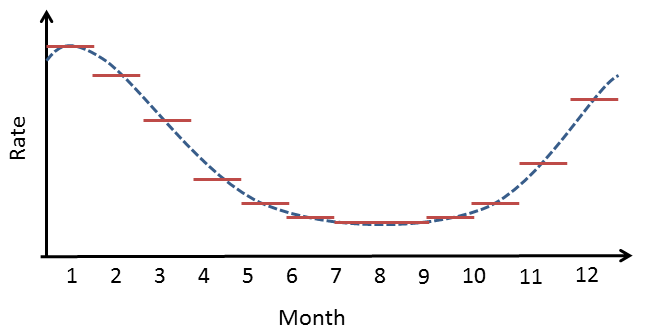
\includegraphics{spline.png} \emph{Figure 1}. Example of how a spline is
used for seasonality: within a month, the risk attributable to
seasonality is assumed to be constant, but from month to month the risks
are assumed to follow a cyclic cubic spline.

Note that the by default all people that have the outcome will be used
to estimate the effect of age and seasonality on the outcome, so not
just the people exposed to the drug of interest. We can add age and
seasonality like this:

\begin{Shaded}
\begin{Highlighting}[]
\NormalTok{ageCovariateSettings <-}\StringTok{ }\KeywordTok{createAgeCovariateSettings}\NormalTok{(}\DataTypeTok{ageKnots =} \DecValTok{5}\NormalTok{)}

\NormalTok{seasonalityCovariateSettings <-}\StringTok{ }\KeywordTok{createSeasonalityCovariateSettings}\NormalTok{(}\DataTypeTok{seasonKnots =} \DecValTok{5}\NormalTok{)}

\NormalTok{sccsIntervalData <-}\StringTok{ }\KeywordTok{createSccsIntervalData}\NormalTok{(}\DataTypeTok{studyPopulation =}\NormalTok{ studyPop,}
                                           \DataTypeTok{sccsData =}\NormalTok{ sccsData,}
                                           \DataTypeTok{eraCovariateSettings =} \KeywordTok{list}\NormalTok{(covarDiclofenacSplit,}
\NormalTok{                                                                       covarPreDiclofenacSplit),}

                                           \DataTypeTok{ageCovariateSettings =}\NormalTok{ ageCovariateSettings,}
                                           \DataTypeTok{seasonalityCovariateSettings =}\NormalTok{ seasonalityCovariateSettings)}
  
\NormalTok{model <-}\StringTok{ }\KeywordTok{fitSccsModel}\NormalTok{(sccsIntervalData)}
\end{Highlighting}
\end{Shaded}

Again, we can inspect the model:

\begin{Shaded}
\begin{Highlighting}[]
\NormalTok{model}
\end{Highlighting}
\end{Shaded}

\begin{verbatim}
## SccsModel object
## 
## Outcome ID: 1
## 
## Outcome count:
##   outcomeSubjects outcomeEvents outcomeObsPeriods
## 1          357183        821368            360559
## 
## Estimates:
## # A tibble: 13 x 7
##    Name                                          ID Estimate LB95CI UB95CI    logRr seLogRr
##    <chr>                                      <dbl>    <dbl>  <dbl>  <dbl>    <dbl>   <dbl>
##  1 Age spline component 1                       100    6.54  NA     NA      1.88    NA     
##  2 Age spline component 2                       101   11.2   NA     NA      2.42    NA     
##  3 Age spline component 3                       102   63.3   NA     NA      4.15    NA     
##  4 Age spline component 4                       103  184.    NA     NA      5.21    NA     
##  5 Age spline component 5                       104 1191.    NA     NA      7.08    NA     
##  6 Seasonality spline component 1               200    0.920 NA     NA     -0.0836  NA     
##  7 Seasonality spline component 2               201    0.923 NA     NA     -0.0798  NA     
##  8 Seasonality spline component 3               202    0.887 NA     NA     -0.119   NA     
##  9 Exposure of interest: Diclofenac, day 0-7   1000    1.28   1.19   1.37   0.245    0.0356
## 10 Exposure of interest: Diclofenac, day 8-14  1001    1.43   1.32   1.54   0.356    0.0391
## 11 Exposure of interest: Diclofenac, day 15-   1002    1.22   1.18   1.26   0.199    0.0181
## 12 Pre-exposure: Diclofenac, day -60--30       1003    1.00   0.964  1.05   0.00451  0.0209
## 13 Pre-exposure: Diclofenac, day -29-          1004    0.934  0.894  0.976 -0.0679   0.0223
\end{verbatim}

We see that our estimates for exposed and pre-exposure time have not
changes much. We can plot the spline curves for age and season to learn
more:

\begin{Shaded}
\begin{Highlighting}[]
\KeywordTok{plotAgeEffect}\NormalTok{(model)}
\end{Highlighting}
\end{Shaded}

\begin{verbatim}
## Warning: Removed 26 row(s) containing missing values (geom_path).
\end{verbatim}

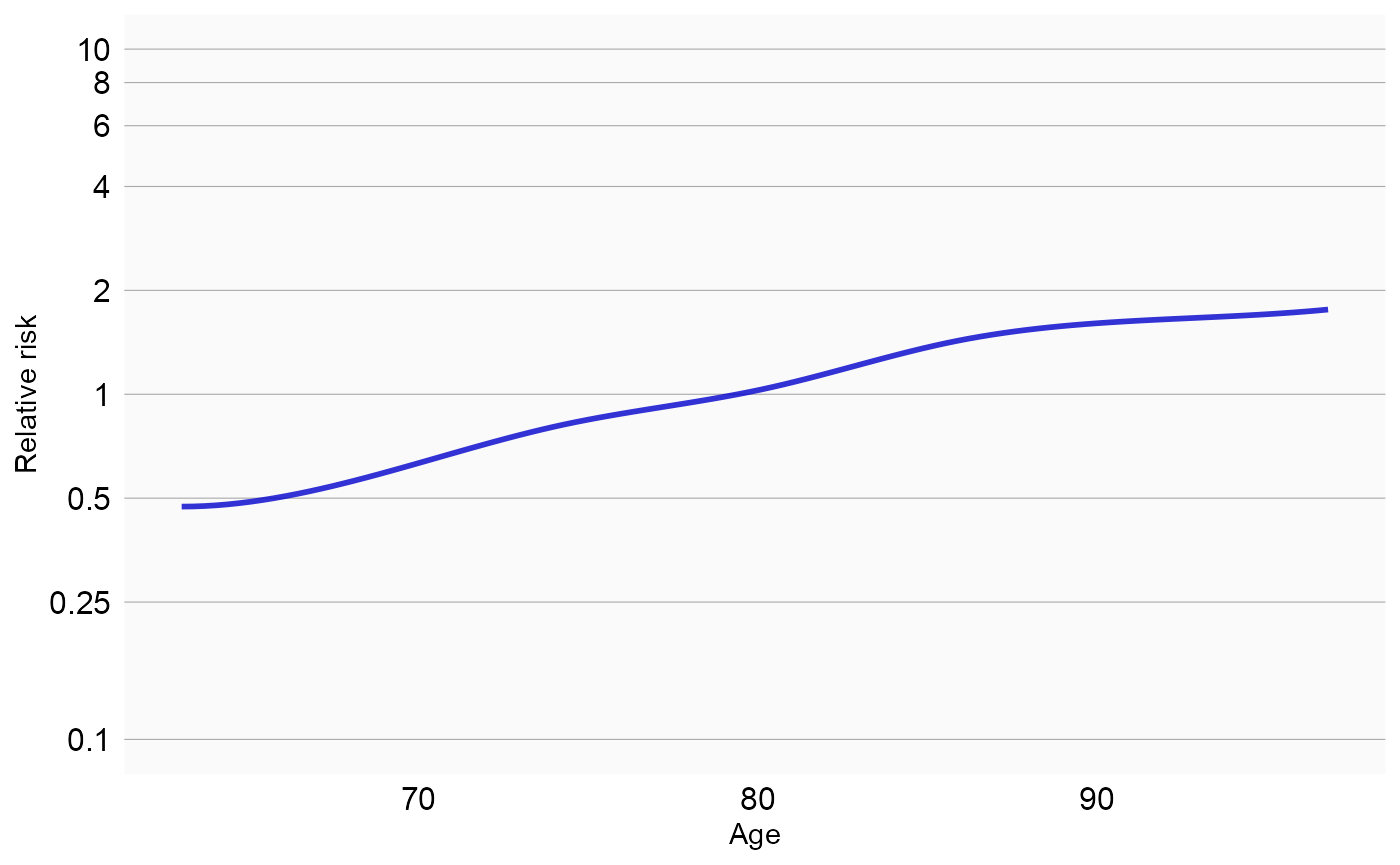
\includegraphics{../inst/doc/SingleStudies_files/figure-latex/unnamed-chunk-33-1.pdf}

\begin{Shaded}
\begin{Highlighting}[]
\KeywordTok{plotSeasonality}\NormalTok{(model)}
\end{Highlighting}
\end{Shaded}

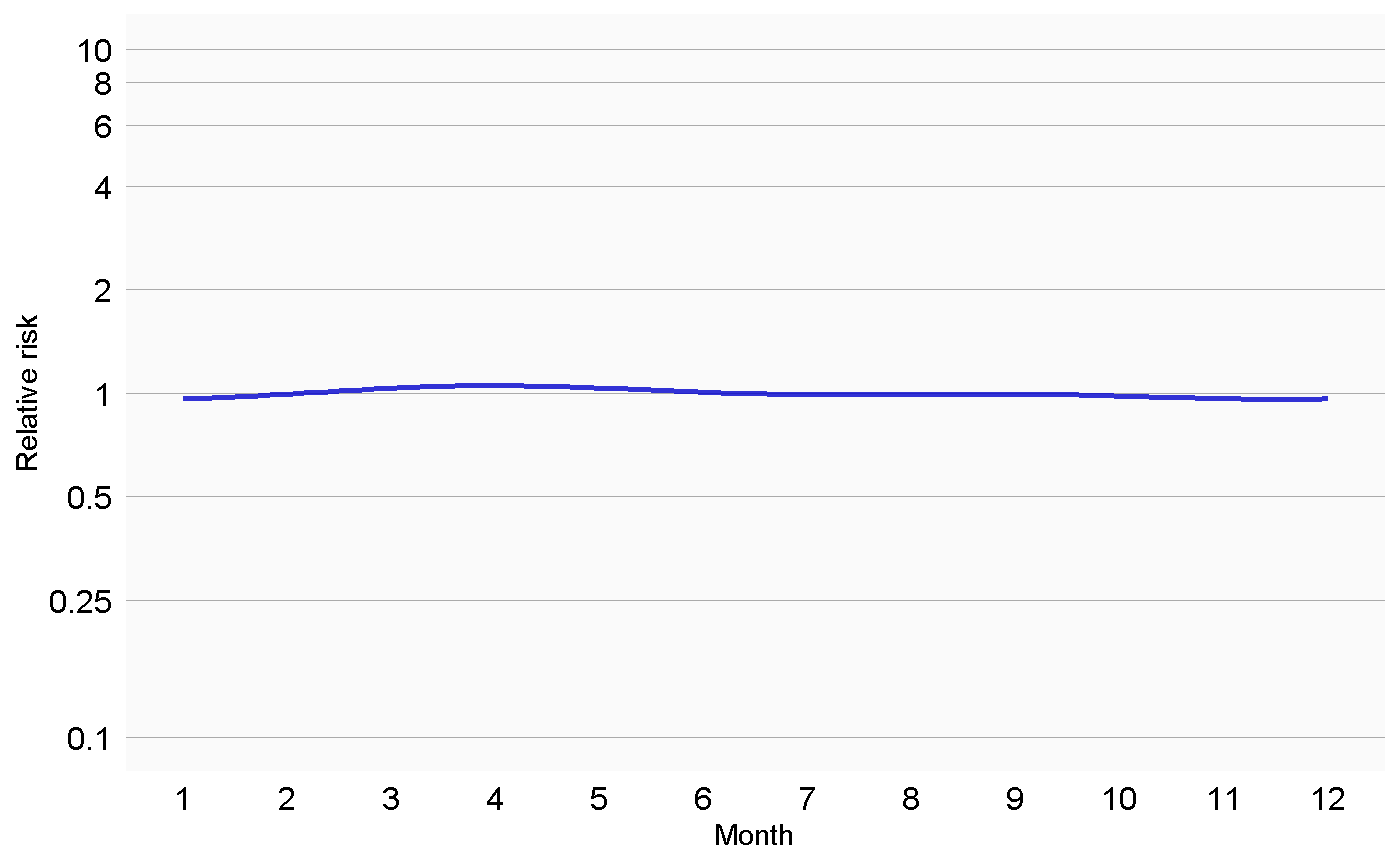
\includegraphics{../inst/doc/SingleStudies_files/figure-latex/unnamed-chunk-35-1.pdf}

We see a strong effect for age on the outcome, but this effect is spread
out over many years and so it less likely to affect the estimates for
any individual, since most people are only observed for a few years in
the database. We do not see a strong effect for season.

\hypertarget{considering-event-dependent-observation-time}{%
\subsection{Considering event-dependent observation
time}\label{considering-event-dependent-observation-time}}

The SCCS method requires that observation periods are independent of
outcome times. This requirement is violated when outcomes increase the
mortality rate, since censoring of the observation periods is then
event-dependent. A modification to the SCCS has been proposed that
attempts to correct for this. First, several models are fitted to
estimate the amount and shape of the event-dependent censoring, and the
best fitting model is selected. Next, this model is used to reweigh
various parts of the observation time. This approach is also implemented
in this package, and can be turned on using the
\texttt{eventDependentObservation} argument of the
\texttt{createSccsIntervalData} function:

\begin{Shaded}
\begin{Highlighting}[]
\NormalTok{sccsIntervalData <-}\StringTok{ }\KeywordTok{createSccsIntervalData}\NormalTok{(}\DataTypeTok{studyPopulation =}\NormalTok{ studyPop,}
                                           \DataTypeTok{sccsData =}\NormalTok{ sccsData,}
                                           \DataTypeTok{eraCovariateSettings =} \KeywordTok{list}\NormalTok{(covarDiclofenacSplit,}
\NormalTok{                                                                       covarPreDiclofenacSplit),}
                                           \DataTypeTok{ageCovariateSettings =}\NormalTok{ ageCovariateSettings,}
                                           \DataTypeTok{seasonalityCovariateSettings =}\NormalTok{ seasonalityCovariateSettings,}
                                           \DataTypeTok{eventDependentObservation =} \OtherTok{TRUE}\NormalTok{)}

\NormalTok{model <-}\StringTok{ }\KeywordTok{fitSccsModel}\NormalTok{(sccsIntervalData)}
\end{Highlighting}
\end{Shaded}

Again, we can inspect the model:

\begin{Shaded}
\begin{Highlighting}[]
\NormalTok{model}
\end{Highlighting}
\end{Shaded}

\begin{verbatim}
## SccsModel object
## 
## Outcome ID: 1
## 
## Outcome count:
##   outcomeSubjects outcomeEvents outcomeObsPeriods
## 1          357183        821368            360559
## 
## Estimates:
## # A tibble: 8 x 7
##   Name                                          ID Estimate LB95CI UB95CI   logRr seLogRr
##   <chr>                                      <dbl>    <dbl>  <dbl>  <dbl>   <dbl>   <dbl>
## 1 Seasonality spline component 1               200    0.926 NA     NA     -0.0772 NA     
## 2 Seasonality spline component 2               201    0.929 NA     NA     -0.0732 NA     
## 3 Seasonality spline component 3               202    0.886 NA     NA     -0.121  NA     
## 4 Exposure of interest: Diclofenac, day 0-7   1000    1.28   1.20   1.38   0.250   0.0356
## 5 Exposure of interest: Diclofenac, day 8-14  1001    1.44   1.33   1.55   0.364   0.0391
## 6 Exposure of interest: Diclofenac, day 15-   1002    1.22   1.17   1.26   0.197   0.0182
## 7 Pre-exposure: Diclofenac, day -60--30       1003    1.03   0.984  1.07   0.0254  0.0211
## 8 Pre-exposure: Diclofenac, day -29-          1004    0.944  0.903  0.986 -0.0578  0.0223
\end{verbatim}

\hypertarget{studies-with-more-than-one-drug}{%
\section{Studies with more than one
drug}\label{studies-with-more-than-one-drug}}

Although we are usually interested in the effect of a single drug or
drug class, it could be beneficial to add exposure to other drugs to the
analysis if we believe those drugs represent time-varying confounders
that we wish to correct for.

\hypertarget{adding-a-class-of-drugs}{%
\subsection{Adding a class of drugs}\label{adding-a-class-of-drugs}}

For example, oftentimes diclofenac is co-prescribed with proton-pump
inhibitors (PPIs) to mitigate the risk of GI bleeding. We would like our
estimate to represent just the effect of the diclofenac, so we need to
keep the effect of the PPIs separate. First we have to retrieve the
information on PPI exposure from the database:

\begin{Shaded}
\begin{Highlighting}[]
\NormalTok{diclofenac <-}\StringTok{ }\DecValTok{1124300}
\NormalTok{ppis <-}\StringTok{ }\KeywordTok{c}\NormalTok{(}\DecValTok{911735}\NormalTok{, }\DecValTok{929887}\NormalTok{, }\DecValTok{923645}\NormalTok{, }\DecValTok{904453}\NormalTok{, }\DecValTok{948078}\NormalTok{, }\DecValTok{19039926}\NormalTok{)}

\NormalTok{sccsData <-}\StringTok{ }\KeywordTok{getDbSccsData}\NormalTok{(}\DataTypeTok{connectionDetails =}\NormalTok{ connectionDetails,}
                          \DataTypeTok{cdmDatabaseSchema =}\NormalTok{ cdmDatabaseSchema,}
                          \DataTypeTok{oracleTempSchema =}\NormalTok{ oracleTempSchema,}
                          \DataTypeTok{outcomeDatabaseSchema =}\NormalTok{ cohortDatabaseSchema,}
                          \DataTypeTok{outcomeTable =}\NormalTok{ outcomeTable,}
                          \DataTypeTok{outcomeIds =} \DecValTok{1}\NormalTok{,}
                          \DataTypeTok{exposureDatabaseSchema =}\NormalTok{ cdmDatabaseSchema,}
                          \DataTypeTok{exposureTable =} \StringTok{"drug_era"}\NormalTok{,}
                          \DataTypeTok{exposureIds =} \KeywordTok{c}\NormalTok{(diclofenac, ppis),}
                          \DataTypeTok{cdmVersion =}\NormalTok{ cdmVersion)}
\NormalTok{sccsData}
\end{Highlighting}
\end{Shaded}

\begin{verbatim}
## # SccsData object
## 
## Exposure cohort ID(s): 1124300,911735,929887,923645,904453,948078,19039926
## Outcome cohort ID(s): 1
## 
## Inherits from Andromeda:
## # Andromeda object
## # Physical location:  C:\Users\MSCHUEMI\AppData\Local\Temp\RtmpiUzJm8\file23f847fa351.sqlite
## 
## Tables:
## $cases (observationPeriodId, caseId, personId, observationDays, startYear, startMonth, startDay, ageInDays, censoredDays, noninformativeEndCensor)
## $eraRef (eraType, eraId, eraName)
## $eras (eraType, caseId, eraId, value, startDay, endDay)
\end{verbatim}

Once retrieved, we can use the data to build and fit our model:

\begin{Shaded}
\begin{Highlighting}[]
\NormalTok{studyPop <-}\StringTok{ }\KeywordTok{createStudyPopulation}\NormalTok{(}\DataTypeTok{sccsData =}\NormalTok{ sccsData,}
                                  \DataTypeTok{outcomeId =} \DecValTok{1}\NormalTok{,}
                                  \DataTypeTok{firstOutcomeOnly =} \OtherTok{FALSE}\NormalTok{,}
                                  \DataTypeTok{naivePeriod =} \DecValTok{180}\NormalTok{)}

\NormalTok{covarPpis <-}\StringTok{ }\KeywordTok{createEraCovariateSettings}\NormalTok{(}\DataTypeTok{label =} \StringTok{"PPIs"}\NormalTok{,}
                                        \DataTypeTok{includeEraIds =}\NormalTok{ ppis,}
                                        \DataTypeTok{stratifyById =} \OtherTok{FALSE}\NormalTok{,}
                                        \DataTypeTok{start =} \DecValTok{1}\NormalTok{,}
                                        \DataTypeTok{end =} \DecValTok{0}\NormalTok{,}
                                        \DataTypeTok{endAnchor =} \StringTok{"era end"}\NormalTok{)}

\NormalTok{sccsIntervalData <-}\StringTok{ }\KeywordTok{createSccsIntervalData}\NormalTok{(}\DataTypeTok{studyPopulation =}\NormalTok{ studyPop,}
                                           \DataTypeTok{sccsData =}\NormalTok{ sccsData,}
                                           \DataTypeTok{eraCovariateSettings =} \KeywordTok{list}\NormalTok{(covarDiclofenacSplit,}
\NormalTok{                                                                       covarPreDiclofenacSplit,}
\NormalTok{                                                                       covarPpis),}
                                           \DataTypeTok{ageCovariateSettings =}\NormalTok{ ageCovariateSettings,}
                                           \DataTypeTok{seasonalityCovariateSettings =}\NormalTok{ seasonalityCovariateSettings,}
                                           \DataTypeTok{eventDependentObservation =} \OtherTok{TRUE}\NormalTok{)}

\NormalTok{model <-}\StringTok{ }\KeywordTok{fitSccsModel}\NormalTok{(sccsIntervalData)}
\end{Highlighting}
\end{Shaded}

Here, we added a new covariate based on the list of concept IDs for the
various PPIs. In this example we set \texttt{stratifyById} to FALSE,
meaning that we will estimate a single incidence rate ratio for all
PPIs, so one estimate for the entire class of drugs. Note that
duplicates will be removed: if a person is exposed to two PPIs on the
same day, this will be counted only once when fitting the model.
Furthermore, we have set the \texttt{start} day to 1 instead of 0. The
reason for this is that PPIs will also be used to treat GI bleeds, and
are likely to be prescribed on the same day as the event. If we would
include day 0, the risk of the outcome would be attributed to the PPI
used for treatment, not the other factors that caused the GI bleed such
as any exposure to our drug of interest. Again, we can inspect the
model:

\begin{Shaded}
\begin{Highlighting}[]
\NormalTok{model}
\end{Highlighting}
\end{Shaded}

\begin{verbatim}
## SccsModel object
## 
## Outcome ID: 1
## 
## Outcome count:
##   outcomeSubjects outcomeEvents outcomeObsPeriods
## 1          357183        821368            360559
## 
## Estimates:
## # A tibble: 9 x 7
##   Name                                          ID Estimate LB95CI UB95CI   logRr  seLogRr
##   <chr>                                      <dbl>    <dbl>  <dbl>  <dbl>   <dbl>    <dbl>
## 1 Seasonality spline component 1               200    0.948 NA     NA     -0.0538 NA      
## 2 Seasonality spline component 2               201    0.934 NA     NA     -0.0687 NA      
## 3 Seasonality spline component 3               202    0.928 NA     NA     -0.0744 NA      
## 4 Exposure of interest: Diclofenac, day 0-7   1000    1.29   1.20   1.38   0.253   0.0355 
## 5 Exposure of interest: Diclofenac, day 8-14  1001    1.44   1.34   1.56   0.368   0.0391 
## 6 Exposure of interest: Diclofenac, day 15-   1002    1.22   1.18   1.27   0.201   0.0183 
## 7 Pre-exposure: Diclofenac, day -60--30       1003    1.03   0.985  1.07   0.0266  0.0209 
## 8 Pre-exposure: Diclofenac, day -29-          1004    0.946  0.905  0.987 -0.0560  0.0223 
## 9 PPIs                                        1005    0.961  0.952  0.969 -0.0401  0.00451
\end{verbatim}

We do see a decrease in risk when people are exposed to PPIs.

\hypertarget{adding-all-drugs}{%
\subsection{Adding all drugs}\label{adding-all-drugs}}

Another approach could be to add all drugs into the model. Again, the
first step is to get all the relevant data from the database:

\begin{Shaded}
\begin{Highlighting}[]
\NormalTok{sccsData <-}\StringTok{ }\KeywordTok{getDbSccsData}\NormalTok{(}\DataTypeTok{connectionDetails =}\NormalTok{ connectionDetails,}
                          \DataTypeTok{cdmDatabaseSchema =}\NormalTok{ cdmDatabaseSchema,}
                          \DataTypeTok{oracleTempSchema =}\NormalTok{ oracleTempSchema,}
                          \DataTypeTok{outcomeDatabaseSchema =}\NormalTok{ cohortDatabaseSchema,}
                          \DataTypeTok{outcomeTable =}\NormalTok{ outcomeTable,}
                          \DataTypeTok{outcomeIds =} \DecValTok{1}\NormalTok{,}
                          \DataTypeTok{exposureDatabaseSchema =}\NormalTok{ cdmDatabaseSchema,}
                          \DataTypeTok{exposureTable =} \StringTok{"drug_era"}\NormalTok{,}
                          \DataTypeTok{exposureIds =} \KeywordTok{c}\NormalTok{(),}
                          \DataTypeTok{cdmVersion =}\NormalTok{ cdmVersion)}
\end{Highlighting}
\end{Shaded}

Note that the \texttt{exposureIds} argument is left empty. This will
cause data for all concepts in the exposure table to be retrieved. Next,
we simply create a new set of covariates, and fit the model:

\begin{Shaded}
\begin{Highlighting}[]
\NormalTok{studyPop <-}\StringTok{ }\KeywordTok{createStudyPopulation}\NormalTok{(}\DataTypeTok{sccsData =}\NormalTok{ sccsData,}
                                  \DataTypeTok{outcomeId =} \DecValTok{1}\NormalTok{,}
                                  \DataTypeTok{firstOutcomeOnly =} \OtherTok{FALSE}\NormalTok{,}
                                  \DataTypeTok{naivePeriod =} \DecValTok{180}\NormalTok{)}

\NormalTok{covarAllDrugs <-}\StringTok{ }\KeywordTok{createEraCovariateSettings}\NormalTok{(}\DataTypeTok{label =} \StringTok{"Other exposures"}\NormalTok{,}
                                            \DataTypeTok{excludeEraIds =}\NormalTok{ diclofenac,}
                                            \DataTypeTok{stratifyById =} \OtherTok{TRUE}\NormalTok{,}
                                            \DataTypeTok{start =} \DecValTok{1}\NormalTok{,}
                                            \DataTypeTok{end =} \DecValTok{0}\NormalTok{,}
                                            \DataTypeTok{endAnchor =} \StringTok{"era end"}\NormalTok{,}
                                            \DataTypeTok{allowRegularization =} \OtherTok{TRUE}\NormalTok{)}

\NormalTok{sccsIntervalData <-}\StringTok{ }\KeywordTok{createSccsIntervalData}\NormalTok{(}\DataTypeTok{studyPopulation =}\NormalTok{ studyPop,}
                                           \DataTypeTok{sccsData =}\NormalTok{ sccsData,}
                                           \DataTypeTok{eraCovariateSettings =} \KeywordTok{list}\NormalTok{(covarDiclofenacSplit,}
\NormalTok{                                                                       covarPreDiclofenacSplit,}
\NormalTok{                                                                       covarAllDrugs),}
                                           \DataTypeTok{ageCovariateSettings =}\NormalTok{ ageCovariateSettings,}
                                           \DataTypeTok{seasonalityCovariateSettings =}\NormalTok{ seasonalityCovariateSettings,}
                                           \DataTypeTok{eventDependentObservation =} \OtherTok{TRUE}\NormalTok{)}

\NormalTok{model <-}\StringTok{ }\KeywordTok{fitSccsModel}\NormalTok{(sccsIntervalData)}
\end{Highlighting}
\end{Shaded}

The first thing to note is that we have defined the new covariates to be
all drugs except diclofenac by not specifying the \texttt{includeEraIds}
and setting the \texttt{excludeEraIds} to the concept ID of diclofenac.
Furthermore, we have specified that \texttt{stratifyById} is TRUE,
meaning an estimate will be produced for each drug.

We have set \texttt{allowRegularization} to TRUE, meaning we will use
regularization for all estimates in this new covariate set.
Regularization means we will impose a prior distribution on the effect
size, effectually penalizing large estimates. This helps fit the model,
for example when some drugs are rare, and when drugs are almost often
prescribed together and their individual effects are difficult to
untangle.

Because there are now so many estimates, we will export all estimates to
a data frame using \texttt{getModel()}:

\begin{Shaded}
\begin{Highlighting}[]
\NormalTok{  estimates <-}\StringTok{ }\KeywordTok{getModel}\NormalTok{(model)}
\NormalTok{  estimates[estimates}\OperatorTok{$}\NormalTok{originalEraId }\OperatorTok{==}\StringTok{ }\NormalTok{diclofenac, ]}
\end{Highlighting}
\end{Shaded}

\begin{verbatim}
## # A tibble: 5 x 10
##   name                                          id estimate lb95Ci ub95Ci    logRr seLogRr originalEraId originalEraType originalEraName
##   <chr>                                      <dbl>    <dbl>  <dbl>  <dbl>    <dbl>   <dbl>         <dbl> <chr>           <chr>          
## 1 Exposure of interest: Diclofenac, day 0-7   1000    1.20   1.11   1.29   0.180    0.0396       1124300 rx              Diclofenac     
## 2 Exposure of interest: Diclofenac, day 8-14  1001    1.37   1.26   1.49   0.317    0.0433       1124300 rx              Diclofenac     
## 3 Exposure of interest: Diclofenac, day 15-   1002    1.19   1.15   1.24   0.176    0.0205       1124300 rx              Diclofenac     
## 4 Pre-exposure: Diclofenac, day -60--30       1003    0.998  0.953  1.04  -0.00245  0.0233       1124300 rx              Diclofenac     
## 5 Pre-exposure: Diclofenac, day -29-          1004    0.911  0.867  0.956 -0.0936   0.0248       1124300 rx              Diclofenac
\end{verbatim}

Here we see that despite the extensive adjustments that are made in the
model, the effect estimates for diclofenac have remained nearly the
same.

In case we're interested, we can also look at the effect sizes for the
PPIs:

\begin{Shaded}
\begin{Highlighting}[]
\NormalTok{estimates[estimates}\OperatorTok{$}\NormalTok{originalEraId }\OperatorTok\StringTok{ }\NormalTok{ppis, ]}
\end{Highlighting}
\end{Shaded}

\begin{verbatim}
## # A tibble: 6 x 10
##   name                                id estimate lb95Ci ub95Ci   logRr seLogRr originalEraId originalEraType originalEraName
##   <chr>                            <dbl>    <dbl>  <dbl>  <dbl>   <dbl>   <dbl>         <dbl> <chr>           <chr>          
## 1 Other exposures: Omeprazole       1076    0.843     NA     NA -0.170       NA        923645 rx              Omeprazole     
## 2 Other exposures: lansoprazole     1204    0.967     NA     NA -0.0340      NA        929887 rx              lansoprazole   
## 3 Other exposures: pantoprazole     1450    0.863     NA     NA -0.147       NA        948078 rx              pantoprazole   
## 4 Other exposures: rabeprazole      1581    0.912     NA     NA -0.0925      NA        911735 rx              rabeprazole    
## 5 Other exposures: Esomeprazole     1897    0.798     NA     NA -0.225       NA        904453 rx              Esomeprazole   
## 6 Other exposures: dexlansoprazole  2327    0.710     NA     NA -0.342       NA      19039926 rx              dexlansoprazole
\end{verbatim}

Note that because we used regularization, we are not able to compute the
confidence intervals for these estimates. We do again see that PPIs all
have relative risks lower than 1 as we would expect.

\hypertarget{diagnostics}{%
\section{Diagnostics}\label{diagnostics}}

We can perform several diagnostics on the data to verify whether our
assumptions underlying the SCCS are met.

\hypertarget{time-from-exposure-start-to-event}{%
\subsection{Time from exposure start to
event}\label{time-from-exposure-start-to-event}}

To gain a better understanding of when the event occurs relative to the
start of exposure, we can plot their relationship. Note that we specify
the naive period, so this can be applied to the data prior to showing
the plot. This will make the plot better in line with the data we ended
up fitting:

\begin{Shaded}
\begin{Highlighting}[]
\KeywordTok{plotExposureCentered}\NormalTok{(studyPop, sccsData, }\DataTypeTok{exposureEraId =}\NormalTok{ diclofenac)}
\end{Highlighting}
\end{Shaded}

\begin{verbatim}
## Warning: Removed 52 rows containing missing values (geom_rect).
\end{verbatim}

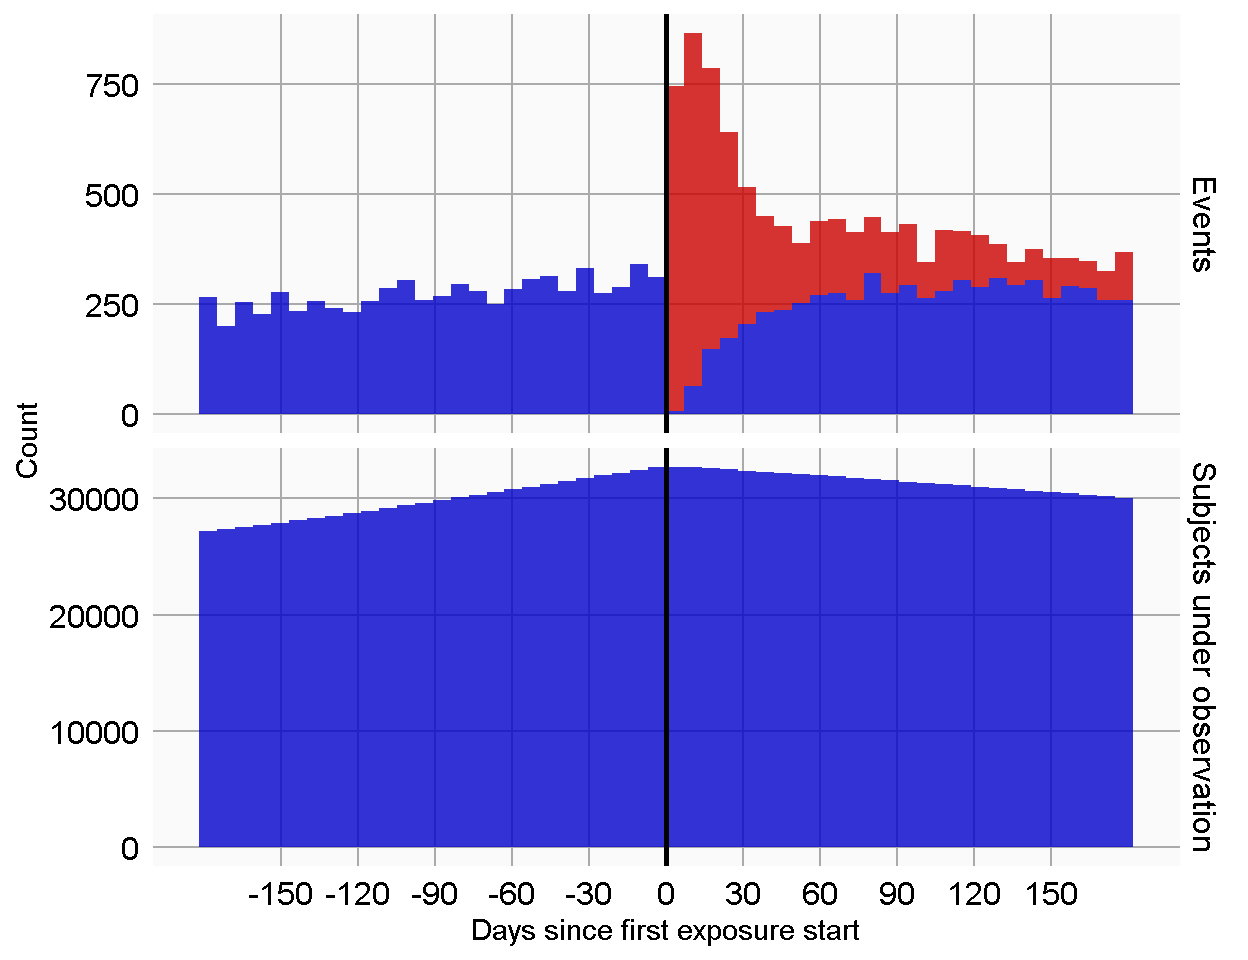
\includegraphics{../inst/doc/SingleStudies_files/figure-latex/unnamed-chunk-52-1.pdf}

This plot suggests an increased rate of events in the first few weeks
following the start of exposure, perhaps because of an acute effect.

\hypertarget{ages-covered-per-subject}{%
\subsection{Ages covered per subject}\label{ages-covered-per-subject}}

We can visualize which age ranges are covered by each subject's
observation time:

\begin{Shaded}
\begin{Highlighting}[]
\KeywordTok{plotAgeSpans}\NormalTok{(studyPop)}
\end{Highlighting}
\end{Shaded}

\begin{verbatim}
## Warning in plotAgeSpans(studyPop): There are 360559 cases. Random sampling 10000 cases.
\end{verbatim}

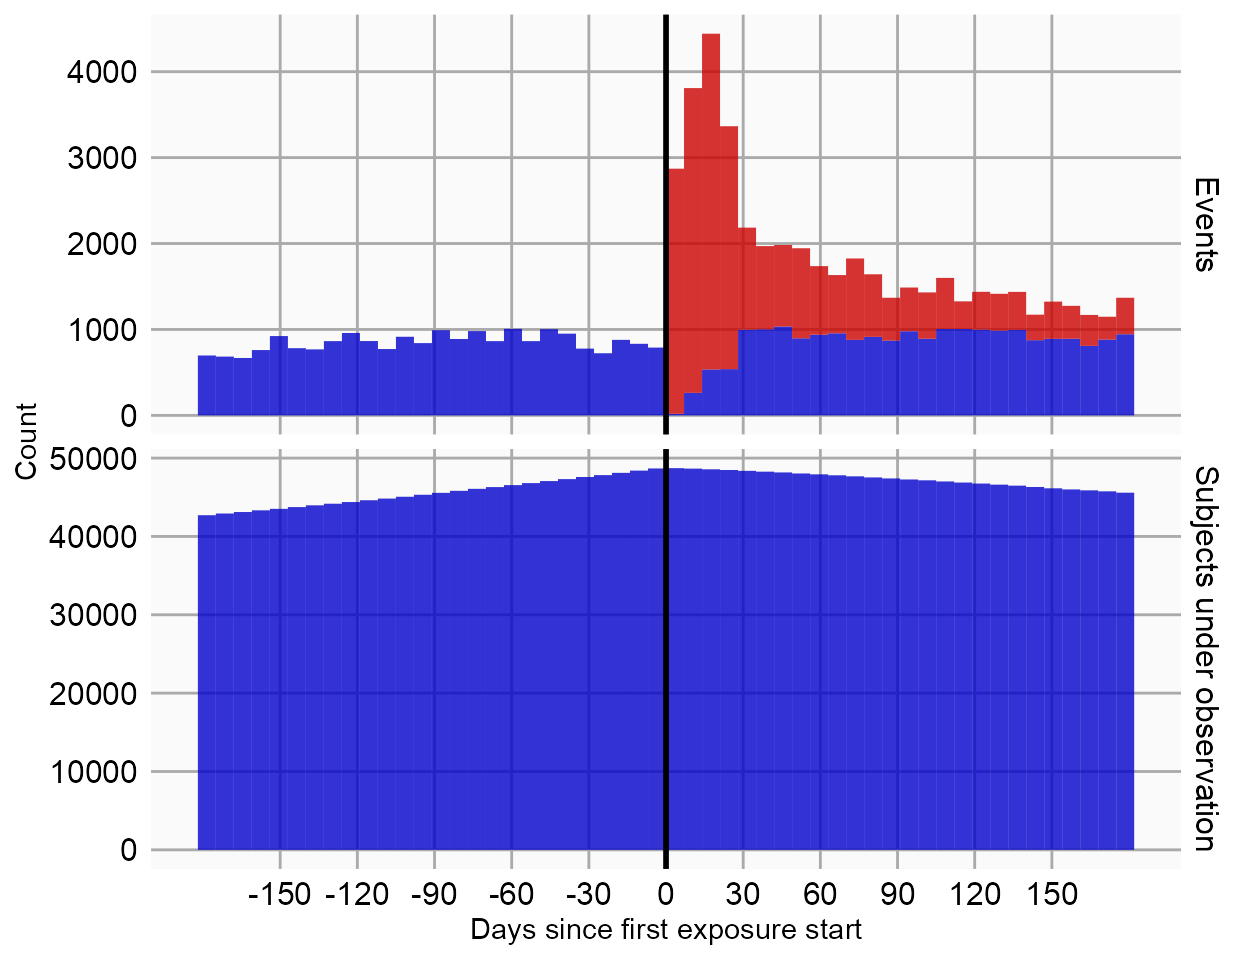
\includegraphics{../inst/doc/SingleStudies_files/figure-latex/unnamed-chunk-54-1.pdf}

Here we see that most observation periods span only a small age range,
making it unlikely that any within-person age-related effect will be
large.

\hypertarget{dependency-between-events-and-observation-end}{%
\subsection{Dependency between events and observation
end}\label{dependency-between-events-and-observation-end}}

To understand whether censoring is dependent on the event, which would
violate one of the assumptions of the SCCS, we can plot the difference
in distribution between censored and uncensored events. By `censored' we
mean periods that end before we would normally expect. Here, we define
periods to be uncensored if they end at either the study end date (if
specified), database end date (i.e.~the date after which no data is
captured in the database), or maximum age (if specified). All other
periods are assumed to be censored.

\begin{Shaded}
\begin{Highlighting}[]
\KeywordTok{plotEventObservationDependence}\NormalTok{(studyPop)}
\end{Highlighting}
\end{Shaded}

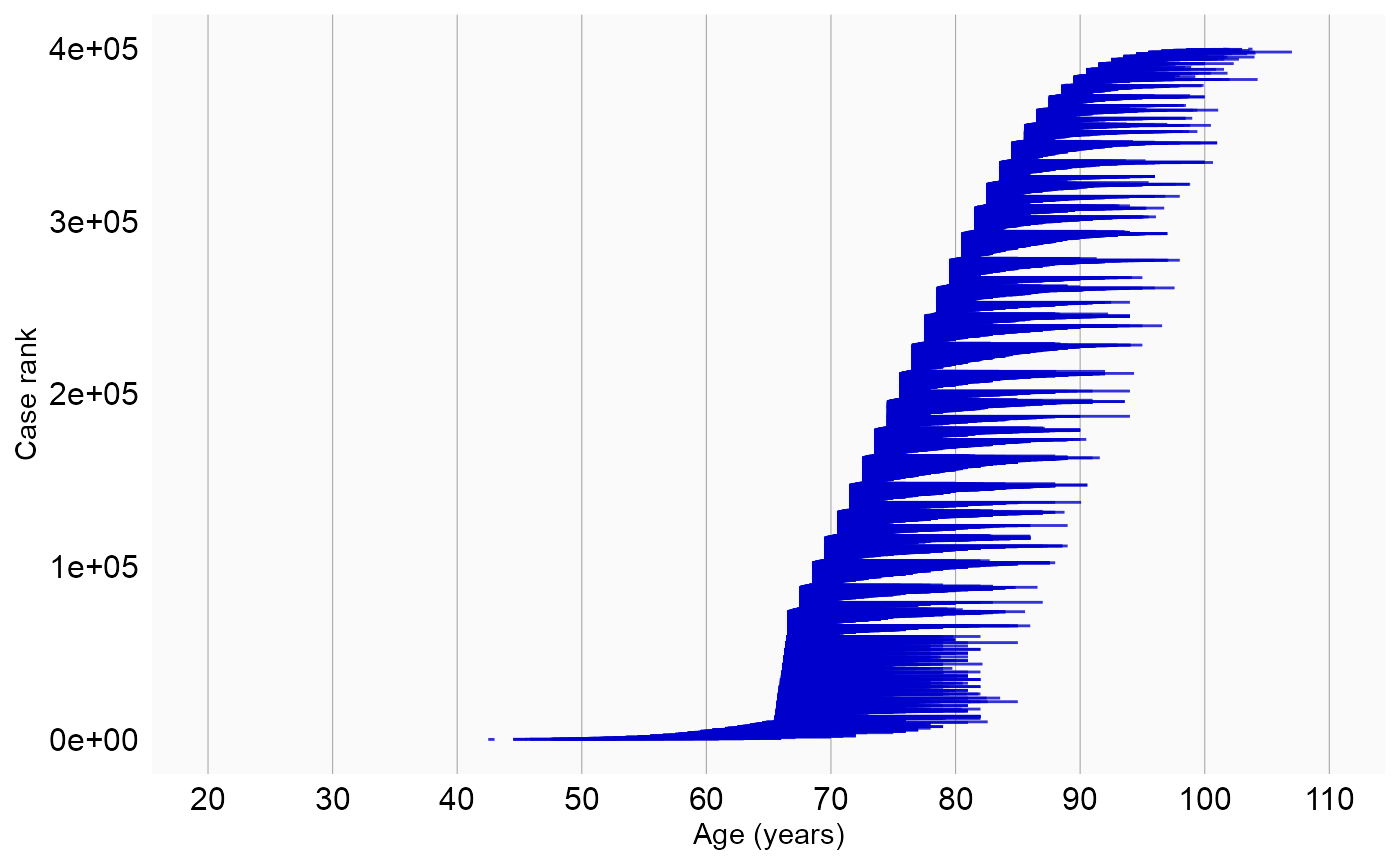
\includegraphics{../inst/doc/SingleStudies_files/figure-latex/unnamed-chunk-56-1.pdf}

Here we see that overall the two distributions are somewhat similar,
with little evidence that censoring tends to lead to shorter times to
the end of observation.

\hypertarget{acknowledgments}{%
\section{Acknowledgments}\label{acknowledgments}}

Considerable work has been dedicated to provide the
\texttt{SelfControlledCaseSeries} package.

\begin{Shaded}
\begin{Highlighting}[]
\KeywordTok{citation}\NormalTok{(}\StringTok{"SelfControlledCaseSeries"}\NormalTok{)}
\end{Highlighting}
\end{Shaded}

\begin{verbatim}
## 
## To cite package 'SelfControlledCaseSeries' in publications use:
## 
##   Martijn Schuemie, Patrick Ryan, Trevor Shaddox and Marc Suchard (2020). SelfControlledCaseSeries: Self-Controlled Case Series. R package version
##   2.0.0. https://github.com/OHDSI/SelfControlledCaseSeries
## 
## A BibTeX entry for LaTeX users is
## 
##   @Manual{,
##     title = {SelfControlledCaseSeries: Self-Controlled Case Series},
##     author = {Martijn Schuemie and Patrick Ryan and Trevor Shaddox and Marc Suchard},
##     year = {2020},
##     note = {R package version 2.0.0},
##     url = {https://github.com/OHDSI/SelfControlledCaseSeries},
##   }
\end{verbatim}

Furthermore, \texttt{SelfControlledCaseSeries} makes extensive use of
the \texttt{Cyclops} package.

\begin{Shaded}
\begin{Highlighting}[]
\KeywordTok{citation}\NormalTok{(}\StringTok{"Cyclops"}\NormalTok{)}
\end{Highlighting}
\end{Shaded}

\begin{verbatim}
## 
## To cite Cyclops in publications use:
## 
## Suchard MA, Simpson SE, Zorych I, Ryan P, Madigan D (2013). "Massive parallelization of serial inference algorithms for complex generalized linear
## models." _ACM Transactions on Modeling and Computer Simulation_, *23*, 10. <URL: http://dl.acm.org/citation.cfm?id=2414791>.
## 
## A BibTeX entry for LaTeX users is
## 
##   @Article{,
##     author = {M. A. Suchard and S. E. Simpson and I. Zorych and P. Ryan and D. Madigan},
##     title = {Massive parallelization of serial inference algorithms for complex generalized linear models},
##     journal = {ACM Transactions on Modeling and Computer Simulation},
##     volume = {23},
##     pages = {10},
##     year = {2013},
##     url = {http://dl.acm.org/citation.cfm?id=2414791},
##   }
\end{verbatim}

Part of the code (related to event-dependent observation periods) is
based on the SCCS package by Yonas Ghebremichael-Weldeselassie, Heather
Whitaker, and Paddy Farrington.

This work is supported in part through the National Science Foundation
grant IIS 1251151.

\end{document}
